% 1998 年全国卷理科第 21 题：等距轨迹曲线段示意图
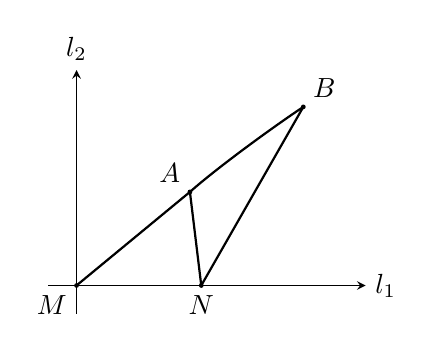
\begin{tikzpicture}[>=stealth, scale=0.72]
  \coordinate (M) at (0,0);
  \coordinate (N) at (2.2,0);
  \coordinate (A) at (2.0,1.65);
  \coordinate (B) at (4.0,3.15);
  \draw[->] (-0.5,0)--(5.1,0) node[right] {$l_1$};
  \draw[->] (0,-0.5)--(0,3.8) node[above] {$l_2$};
  \draw[thick] (A) .. controls (2.45,2.05) and (3.4,2.75) .. (B);
  \draw[thick] (A)--(M) (A)--(N) (B)--(N);
  \draw[dashed] (M)--(A);
  \fill (M) circle (1.2pt) node[below left] {$M$};
  \fill (N) circle (1.2pt) node[below] {$N$};
  \fill (A) circle (1.2pt) node[above left] {$A$};
  \fill (B) circle (1.2pt) node[above right] {$B$};
\end{tikzpicture}
